\chapter{Zaključak}

Svi dosadašnji eksperimeni kojima su testirane Belove nejednakosti su pokazali da su one narušene, što predstavlja eksperimentalnu potvrdu ispravnosti kvantne mehanike i propast "realizma" zbog njegove pretpostavke o lokalnosti.

S druge strane ideja o nelokalnosti (u kontekstu superluminalnog uticaja) je svakako uznemiruju\' ca jer je toliko druga\v cija od onoga \v sto nam intuicija govori i ima neprihvatljive implikacije.
Prema specijalnoj teoriji relativnosti, postoje inercijalni sistemi u kojima se takav signal \v siri unazad u vremenu, pa bi efekti prethodili sopstvenim uzrocima - \v sto dovodi do
razli\v citih logi\v ckih anomalija.
Pitanje je da li su efekti posmatrani u ovim eksperimentima kauzalni, ili su dovoljno eteri\v cni da se izbjegne filozofski odgovor i da superluminalni uticaji u tom slu\v caju
dobiju novi interpretaciju.

Jedan od takvih primjera eteri\v cnih efekata bila bi sjenka bube koja preleti preko svjetlosnog snopa filmskog projektora (slika \ref{fig:bug_on_screen}). Udaljenost do ekrana mo\v ze biti proizvoljna, pa samim tim i brzina sjenke
mo\v ze biti proizvoljno velika, tako da mo\v zemo zamisliti scenario u kojem se sjenka bube kre\' ce brzinom ve\' com od brzine svjetlosti.
Ono \v sto ovdje moramo primjetiti je da sjenka ne nosi nikakvu energiju, niti prenosi bilo kakvu informaciju s jedne ta\v cke na drugu, tako da mi ne mo\v zemo iz ta\v cke $X$ prouzrokovati bilo
\v sta u ta\v cki $Y$ manipulacijom prolazne sjenke.

\begin{figure}[H]
    \centering
    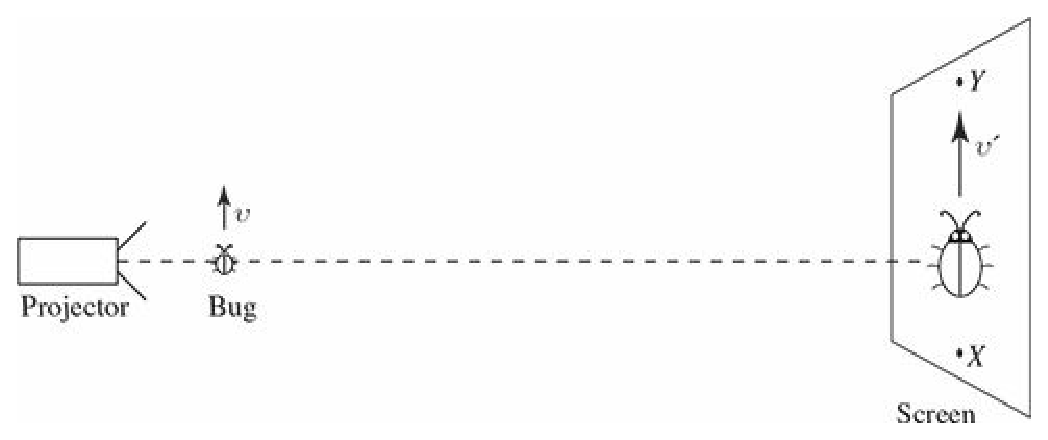
\includegraphics[width=0.75\textwidth]{figures/bug_on_screen.eps}
    \caption{Buba se kre\' ce brzinom $v$ preko svjetlosnog snopa filmskog projektora. U zavisnosti od udaljenosti platna, brzina $v'$ mo\v ze biti proivoljno velika.}
    \label{fig:bug_on_screen}
\end{figure}

O\v cigledno je da u Belovom eksperimentu postoji korelacija u podacima, s tim \v sto tu korelaciju mo\v zemo da vidimo
samo nakon \v sto uporedimo dva seta podataka (nakon \v sto su oba mjerenja zavr\v sena).
U skladu sa tim, odgovor na pitanje: "Da li mjerenje elektrona uti\v ce na sa njim spregnuti pozitron", je {\it{da}}, ali ne u obi\v cnom smislu te rije\v ci.
Da je odgovor negativan, ne bismo mogli objasniti korelacije u podacima.

Osoba koja vr\v si eksperiment, mo\v ze jedino da kontroli\v se da li \' ce izvr\v siti mjerenje ili ne, ali ne mo\v ze uticati na njegov ishod i ti rezultati su prakti\v cno
nasumi\v cni (ako se posmatraju odvojeno od rezulatata eksperimenata sa spregnutom \v cesticom) i ona ne mo\v ze koristiti svoje mjerenje da po\v salje signal osobi
na detektoru spregnute \v cestice (ne mo\v ze natjerati datu \v cesticu da promijeni spin, kao \v sto ni osoba u $X$ ne mo\v ze da uti\v ce na sjenku bube).

Ovo nas navodi da razlikujemo dvije vrste uticaja: "uzro\v cne" vrste i "eteri\v cne" vrste.
Uzro\v cne mo\v zemo detektovati vr\v se\' ci mjerenje na samom podsistemu, dok je za eteri\v cne, koje ne prenose informacije ili energiju, jedini dokaz
korelacija u podacima dobijenim eksperimentima na dva razli\v cita podsistema.
Uzro\v cni uticaji se ne mogu \v siriti superluminalnim brzinama, tj. princip lokalnosti za njih i dalje važi, ali zasad ne postoji razlog za\v sto bi to moralo da va\v zi za eteri\v cne.